\subsection{JQC-3FF-S-Z -- Relai Daya}
\label{subsec:jqc-3ff-s-z}

% ---------------------------------------------------------------------
\subsubsection{Identitas dan Fungsi}
\begin{wrapfigure}{r}{0.3\textwidth}% 'r' untuk posisi kanan, '0.25\textwidth' untuk lebar gambar
	\vspace{-15pt}
	\centering
	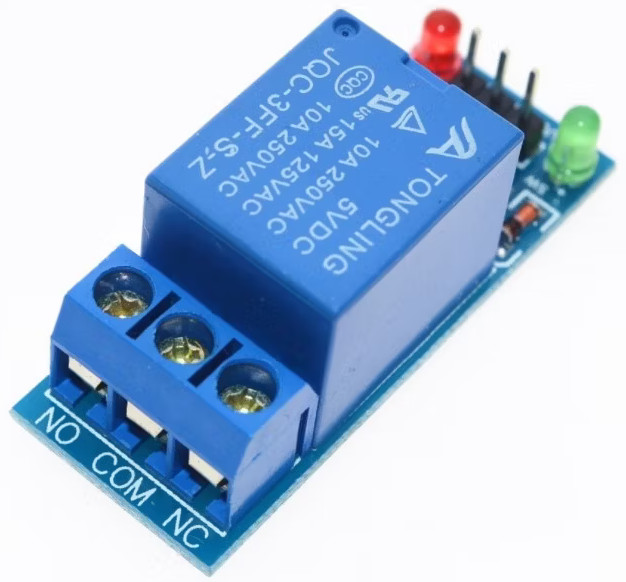
\includegraphics[width=\linewidth]{images/jqc_power_relay.jpg} % Ganti dengan nama file gambar Anda
	\caption{Relai daya JQC-3FF-S-Z.}
	\label{fig:jqc-3ff-power_relay}
\end{wrapfigure}

Modul relai daya JQC-3FF-S-Z adalah aktuator sakelar elektromekanis yang berfungsi sebagai antarmuka isolasi dan pengendali daya antara sirkuit kontrol berdaya rendah (mikrokontroler) dengan beban beban listrik bertegangan dan berarus tinggi (AC atau DC). Dalam sistem tertanam, relai dikategorikan sebagai aktuator switching terisolasi.

Modul relai JQC-3FF-S-Z memiliki ketahanan beban kontak hingga $10\,\text{A}$, integrasi komponen isolasi optik (\textit{optocoupler}) PC817 untuk melindungi jalur utama mikrokontroler dari interferensi lonjakan tegangan balik (\textit{back-EMF}), serta kompatibilitas pemicuan logika kontrol secara langsung dari pin GPIO mikrokontroler $3{,}3\,\text{V}$ maupun $5\,\text{V}$.

\begin{table}[H]
	\centering
	\caption{Identitas komponen modul relai JQC-3FF-S-Z}
	\label{tab:jqc3ff_identitas}
	\small
	\begin{tabularx}{\textwidth}{@{} p{3.8cm} X @{}}
		\toprule
		Parameter          & Keterangan                                                                                                                   \\
		\midrule
		Nama komponen      & Modul Relai Daya 1-Saluran dengan Optocoupler (\textit{1-Channel Relay Module})                                              \\
		Model/part number  & JQC-3FF-S-Z (Elektromekanis) / PC817 (Optocoupler Driver)                                                                    \\
		Jenis              & Aktuator Elektromekanis / Sakelar Terisolasi Optik                                                                           \\
		Fungsi utama       & Pengendali sakelar beban tegangan tinggi ($250\,\text{V AC} / 30\,\text{V DC}$) melalui sinyal logika kontrol berdaya rendah \\
		Sumber dokumentasi & JQC-3FF-S-Z Datasheet (Datasheet4u)                            \\
		\bottomrule
	\end{tabularx}
\end{table}

% ---------------------------------------------------------------------
\subsubsection{Prinsip Kerja}
Cara kerja modul relai JQC-3FF-S-Z pada dasarnya menyerupai sakelar otomatis yang digerakkan oleh magnet (\textit{elektromagnet}) dan dilindungi oleh sinyal optik (\textit{optocoupler}). Struktur internal modul ini terbagi menjadi dua bagian utama:

\begin{enumerate}
	\item \textbf{Bagian Sakelar Mekanis dan Magnet (Koil \& Lidah Kontak):}
	      Di dalam modul relai terdapat koil kawat tembaga yang melilit sebuah inti besi. Saat arus listrik mengalir melewati koil tersebut, inti besi berubah menjadi magnet sementara. Medan magnet ini menarik tuas atau lidah kontak mekanis (\textit{armature}) sehingga posisi sakelar berpindah dari posisi awal \textit{Normally Closed} (NC / terhubung saat mati) menuju posisi \textit{Normally Open} (NO / terhubung saat aktif). Ketika arus listrik ke koil dihentikan, magnet hilang dan pegas internal langsung mengembalikan sakelar ke posisi awal (NC).

	      \begin{figure}[H]
		      \centering
		      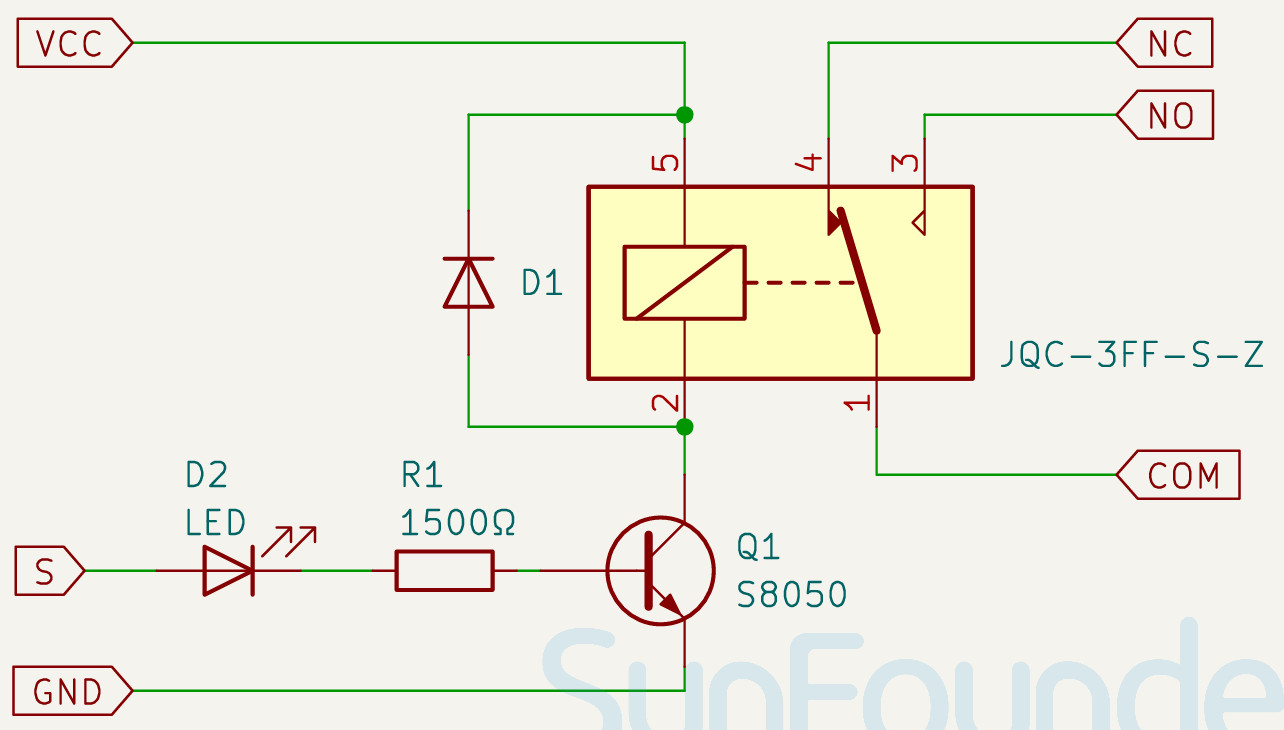
\includegraphics[width=0.55\textwidth]{images/relay_module_schematic.jpg}
		      % \fbox{\parbox[c][3.5cm][c]{0.55\textwidth}{\centering Diagram Blok Internal Modul Relai: Sinyal IN $\rightarrow$ Optocoupler PC817 $\rightarrow$ Transistor Driver $\rightarrow$ Koil JQC-3FF $\rightarrow$ Terminal Kontak (NO/COM/NC)}}
		      \caption{Struktur fungsional internal modul relai JQC-3FF-S-Z terisolasi optik.}
		      \label{fig:jqc3ff_karakteristik}
	      \end{figure}

	\item \textbf{Bagian Pengaman dan Penggerak Sinyal (Optocoupler \& Transistor):}
	      Koil relai membutuhkan arus sekitar $70\,\text{mA}$ untuk dapat menarik sakelar. Arus ini terlalu besar jika diambil langsung dari pin mikrokontroler (yang umumnya hanya mampu memproses $\approx 20\text{--}40\,\text{mA}$). Oleh karena itu, modul ini dilengkapi komponen pengaman berupa \textit{optocoupler} PC817 dan transistor driver:
	      \begin{itemize}
		      \item Pin mikrokontroler hanya perlu menyalakan lampu LED inframerah kecil di dalam \textit{optocoupler}.
		      \item Cahaya dari LED tersebut ditangkap oleh sensor cahaya (\textit{fototransistor}) di dalamnya untuk memicu transistor penggerak utama, yang kemudian menyalurkan arus daya $5\,\text{V}$ menuju koil relai.
		      \item Komponen diode pemintas (\textit{flyback diode}) dipasang secara sejajar pada koil untuk menyerap kejutan listrik balik (\textit{back-EMF}) yang timbul saat relai dimatikan, sehingga sirkuit kontrol tetap aman dari lonjakan tegangan.
	      \end{itemize}
\end{enumerate}

\paragraph{Konsep dan Formulasi Matematis Terkait}
Gaya magnetik $F_m$ yang dihasilkan oleh koil relai untuk menarik jangkar mekanis berbanding lurus dengan kuadrat arus koil $I$, jumlah lilitan $N$, dan luas penampang inti magnetik $A$, yang dirumuskan sebagai:

\begin{equation}
	F_m = \frac{\mu_0 \cdot (N \cdot I)^2 \cdot A}{2 \cdot g^2}
	\label{eq:jqc3ff_gaya_magnet}
\end{equation}

\noindent di mana:
\begin{itemize}
	\item $F_m$ = Gaya tarik elektromagnetik pada jangkar ($\text{N}$).
	\item $\mu_0$ = Permeabilitas vakum/udara ($4\pi \times 10^{-7}\,\text{H/m}$).
	\item $N$ = Jumlah lilitan kawat pada koil relai.
	\item $I$ = Arus listrik yang mengalir melalui koil ($\text{A}$).
	\item $A$ = Luas penampang inti besi elektromagnet ($\text{m}^2$).
	\item $g$ = Lebar celah udara (\textit{air gap}) antara jangkar dan inti besi ($\text{m}$).
\end{itemize}

% ---------------------------------------------------------------------
\subsubsection{Alur Kerja Internal dan Protokol Komunikasi}
Alur pemrosesan operasional modul relai mengikuti pola \textbf{Input $\rightarrow$ Proses $\rightarrow$ Output}:
\begin{enumerate}
	\item \textbf{Input:} Perubahan kondisi logika digital ($0\,\text{V}$ LOW atau $5\,\text{V}$ HIGH) dari pin GPIO mikrokontroler menuju pin masukan kontrol (\texttt{IN}).
	\item \textbf{Proses:} Pancaran cahaya inframerah dari LED internal \textit{optocoupler} PC817 mengaktifkan fototransistor di dalamnya. Sinyal ini kemudian memicu transistor penggerak utama hingga aktif sepenuhnya (\textit{ON}), sehingga arus listrik mengalir menuju koil relai JQC-3FF.
	\item \textbf{Output:} Pergerakan lidah kontak mekanis yang menghubungkan terminal \textit{Common} (COM) ke \textit{Normally Open} (NO) atau \textit{Normally Closed} (NC), yang berfungsi mengalirkan atau memutuskan arus listrik pada beban eksternal.
\end{enumerate}

\paragraph{Detail Sinyal Kontrol}
Modul relai tidak menggunakan protokol komunikasi data serial, melainkan dikendalikan secara langsung melalui sinyal logika biner (\textit{Discrete Digital Control}):
\begin{itemize}
	\item \textbf{Mode Pemicuan (\textit{Active-LOW}):} Modul relai terisolasi \textit{optocoupler} ini beroperasi dengan logika \textit{Active-LOW}. Pemicuan terjadi ketika mikrokontroler menarik pin \texttt{IN} ke logika LOW ($0\,\text{V}$). Kondisi ini menciptakan beda potensial yang menyalakan LED internal \textit{optocoupler} sehingga koil relai teraliri listrik.
	\item \textbf{Waktu Pembukaan/Penutupan Mekanis (\textit{Operate \& Release Time}):} Karena relai menggunakan komponen mekanis (lidah kontak), terdapat jeda waktu fisik saat kontak berpindah posisi:
	      \begin{itemize}
		      \item \textbf{Jeda Kontak Penutupan (\textit{Operate Delay}):} Membutuhkan waktu $\approx 10\,\text{ms}$ sejak pin \texttt{IN} diberi sinyal LOW hingga kontak COM dan NO terhubung rapat.
		      \item \textbf{Jeda Pelepasan Kontak (\textit{Release Delay}):} Membutuhkan waktu $\approx 5\,\text{ms}$ sejak pin \texttt{IN} kembali ke HIGH hingga pegas internal mengembalikan kontak ke posisi awal (NC).
	      \end{itemize}
\end{itemize}

\begin{figure}[htbp]
	\centering
	\begin{tikzpicture}[x=0.18mm, y=10mm, >=Stealth, font=\sffamily\small]
		% Axis Utama
		\draw[->, color=gray!60, thick] (0, 0) -- (600, 0) node[right, color=black] {\textit{Waktu}};
		\draw[->, color=gray!60, thick] (0, 0) -- (0, 2.5) node[above, color=black] {Kondisi Logika};

		% Level Logika
		\node[left, font=\scriptsize] at (0, 1.8) {\textbf{HIGH (5V)}};
		\node[left, font=\scriptsize] at (0, 0.4) {\textbf{LOW (0V)}};
		\draw[dotted, color=gray!40] (0, 1.8) -- (580, 1.8);
		\draw[dotted, color=gray!40] (0, 0.4) -- (580, 0.4);

		% Gelombang Sinyal Kontrol IN (Active-LOW)
		% Transisi LOW di x = 60, Kembali HIGH di x = 360
		\draw[ultra thick, color={rgb,255:red,30;green,64;blue,175}]
		(0, 1.8) -- (60, 1.8) -- (60, 0.4) -- (360, 0.4) -- (360, 1.8) -- (580, 1.8);
		\node[color={rgb,255:red,30;green,64;blue,175}, font=\tiny\bfseries, above] at (30, 1.8) {IN: Standby (HIGH)};
		\node[color={rgb,255:red,30;green,64;blue,175}, font=\tiny\bfseries, below] at (210, 0.4) {IN: Pemicuan (LOW)};

		% Gelombang Respons Kontak COM-NO (Diperlebar rentang delay-nya secara visual)
		% Transisi ON di x = 150 (jarak 90 unit), Transisi OFF di x = 440 (jarak 80 unit)
		\draw[thick, color={rgb,255:red,217;green,119;blue,6}, dash pattern=on 4pt off 2pt]
		(0, 0.4) -- (150, 0.4) -- (150, 1.8) -- (440, 1.8) -- (440, 0.4) -- (580, 0.4);

		% Garis Bantu Vertikal Putus-Putus
		\draw[dashed, color=gray!50] (60, 1.8) -- (60, 0.2);
		\draw[dashed, color=gray!50] (150, 1.8) -- (150, 0.2);
		\draw[dashed, color=gray!50] (360, 1.8) -- (360, 0.2);
		\draw[dashed, color=gray!50] (440, 1.8) -- (440, 0.2);

		% Anotasi Delay (Diperlebar sehingga text width & shortstack muat sempurna)
		\draw[stealth-stealth, color=red!80!black, thick] (60, 1.1) -- (150, 1.1)
		node[midway, below, font=\tiny, align=center] {\shortstack{\textit{Operate Delay}\\$\approx 10\,\text{ms}$}};
		\draw[stealth-stealth, color=red!80!black, thick] (360, 1.1) -- (440, 1.1)
		node[midway, below, font=\tiny, align=center] {\shortstack{\textit{Release Delay}\\$\approx 5\,\text{ms}$}};

		% Label Status Kontak
		\node[color={rgb,255:red,217;green,119;blue,6}, font=\tiny\bfseries, above] at (295, 1.8) {Kontak COM-NO: Tertutup (ON)};
	\end{tikzpicture}
	\caption{Diagram pewaktu sinyal kontrol pemicuan \textit{Active-LOW} dan respons tanggapan kontak mekanis relai JQC-3FF-S-Z.}
	\label{fig:jqc3ff_timing}
\end{figure}

% ---------------------------------------------------------------------
\subsubsection{Besaran yang Diukur atau Dikendalikan}
Relai JQC-3FF-S-Z bertindak sebagai pengendali sakelar daya listrik berkapasitas besar. Parameter batas operasional switching relai dirangkum pada Tabel~\ref{tab:jqc3ff_karakteristik_besaran}.

\begin{table}[H]
	\centering
	\caption{Karakteristik besaran operasional relai JQC-3FF-S-Z}
	\label{tab:jqc3ff_karakteristik_besaran}
	\small
	\begin{tabularx}{\textwidth}{@{} p{3.8cm} >{\hsize=0.7\hsize}X >{\hsize=1.3\hsize}X @{}}
		\toprule
		Parameter               & Nilai                                                                          & Keterangan                                          \\
		\midrule
		Besaran Utama           & Tegangan \& Arus Daya Beban                                                    & Sakelar daya biner terisolasi (\textit{Open/Close}) \\
		Kapasitas Beban AC      & Maksimum $250\,\text{V AC} / 10\,\text{A}$                                     & Batas aman switching beban arus bolak-balik         \\
		Kapasitas Beban DC      & Maksimum $30\,\text{V DC} / 10\,\text{A}$                                      & Batas aman switching beban arus searah              \\
		Resistansi Kontak Awal  & $\le 100\,\text{m}\Omega$                                                      & Resistansi antar-terminal kontak saat terhubung     \\
		Masa Pakai Mekanis      & $10.000.000$ kali operasi                                                      & Siklus peralihan sakelar tanpa beban listrik        \\
		Masa Pakai Elektrik     & $100.000$ kali operasi                                                         & Siklus peralihan sakelar pada beban penuh terpasang \\
		Waktu Respons Switching & $\le 10\,\text{ms}$ (\textit{Operate}) / $\le 5\,\text{ms}$ (\textit{Release}) & Kecepatan pergerakan lidah kontak mekanis           \\
		\bottomrule
	\end{tabularx}
\end{table}

% ---------------------------------------------------------------------
\subsubsection{Karakteristik Sinyal}
Sinyal kontrol yang diterima oleh modul relai berupa logika tegangan diskret murni yang mengendalikan isolator optik internal.

\begin{table}[H]
	\centering
	\caption{Karakteristik sinyal kontrol modul relai JQC-3FF-S-Z}
	\label{tab:jqc3ff_sinyal}
	\small
	\begin{tabularx}{\textwidth}{@{} p{3.8cm} >{\hsize=0.8\hsize}X >{\hsize=1.2\hsize}X @{}}
		\toprule
		Aspek                     & Nilai                                                 & Keterangan                                                           \\
		\midrule
		Jenis Sinyal              & Sinyal Logika Digital Diskret                         & Kontrol Biner ($0$ / $1$) pemicu optocoupler                         \\
		Tegangan Logika Pemicu    & $0\text{--}5\,\text{V DC}$ (TTL / CMOS)               & Kompatibel dengan sinyal kontrol $3{,}3\,\text{V}$ dan $5\,\text{V}$ \\
		Arus Pemicu Pin IN        & $2\text{--}5\,\text{mA}$ per saluran                  & Arus sangat rendah, aman untuk pin GPIO MCU                          \\
		Tipe Pemicuan             & \textit{Active-LOW} (bawaan modul)                    & Relai aktif saat pin IN ditarik ke $0\,\text{V}$ (GND)               \\
		Isolasi Tegangan          & $5.000\,\text{V}_{\text{RMS}}$ (\textit{Optocoupler}) & Mengisolasi total jalur kontrol dari bus daya beban                  \\
		Frekuensi Switching Maks. & $\le 20\,\text{Hz}$                                   & Dibatasi oleh inersia massa mekanis kontak relai                     \\
		\bottomrule
	\end{tabularx}
\end{table}

% ---------------------------------------------------------------------
\subsubsection{Pin, Catu Daya, dan Antarmuka}
Modul relai JQC-3FF-S-Z dikemas dalam papan pengembang (\textit{breakout board}) yang memisahkan sisi kendali sinyal berdaya rendah (\textit{header pin}) dengan sisi beban tegangan tinggi (\textit{screw terminal block}).

\begin{figure}[H]
	\centering
	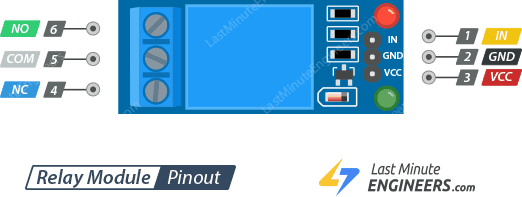
\includegraphics[width=0.5\textwidth]{images/one-channel-relay-module-pinout.png}
	\caption{Pemetaan pin dan antarmuka modul JQC-3FF-S-R relai daya.}
	\label{fig:jqc-3ff-s-r_interface}
\end{figure}

\begin{table}[H]
	\centering
	\caption{Pemetaan pin antarmuka modul relai JQC-3FF-S-Z}
	\label{tab:jqc3ff_pin}
	\small
	\begin{tabularx}{\textwidth}{@{} p{3.2cm} p{2.5cm} X @{}}
		\toprule
		Pin (Modul Breakout)          & Fungsi            & Keterangan                                                       \\
		\midrule
		VCC                           & $V_{CC}$          & Catu daya positif sirkuit driver ($\text{4{,}5--5\,V DC}$)       \\
		IN                            & Sinyal Kontrol    & Pin pemicu logika dari GPIO mikrokontroler                       \\
		GND                           & GND               & Referensi ground ($0\,\text{V}$)                                 \\
		\midrule
		NO (\textit{Normally Open})   & Kontak Beban      & Terhubung ke COM hanya saat relai dipicu (aktif)                 \\
		COM (\textit{Common})         & Jalur Utama Beban & Terminal pusat yang dihubungkan ke salah satu fasa beban         \\
		NC (\textit{Normally Closed}) & Kontak Beban      & Terhubung ke COM secara otomatis saat relai mati (\textit{idle}) \\
		\bottomrule
	\end{tabularx}
\end{table}

\subsubsection{Kebutuhan Catu Daya}
Koil relai JQC-3FF-S-Z beroperasi pada tegangan $5\,\text{V DC}$ dengan konsumsi arus sekitar $70\,\text{mA}$ saat relai aktif (sakelar tertarik). Saat kondisi siaga (\textit{standby} / relai mati), konsumsi arusnya sangat kecil hingga mendekati $0\,\text{mA}$. Karena kebutuhan arus $70\,\text{mA}$ ini cukup besar untuk ukuran aktuator kecil, pasokan daya pin \texttt{VCC} (atau \texttt{JD-VCC}) sebaiknya dihubungkan langsung ke saluran daya utama $5\,\text{V}$ mikrokontroler atau menggunakan adaptor eksternal, bukan dari pin luaran regulator yang kapasitas arusnya terbatas.

Pada sisi sinyal kontrol, integrasi \textit{optocoupler} PC817 membuat pin pemicu \texttt{IN} dapat merespons sinyal logika $3{,}3\,\text{V}$ (seperti dari ESP32 atau STM32) maupun $5\,\text{V}$ (seperti dari Arduino Mega 2560) secara langsung tanpa membutuhkan konverter level logika (\textit{logic level converter}). Selain itu, papan pengembang (\textit{breakout board}) modul ini sudah dilengkapi diode pemintas (\textit{flyback diode}) yang dipasang sejajar dengan koil untuk menyerap lonjakan tegangan induksi saat relai dimatikan, sehingga komponen elektronika di sekitarnya tetap aman.

% ---------------------------------------------------------------------
\subsubsection{Spesifikasi Penting dari Datasheet}
Rangkuman parameter teknis operasional modul relai JQC-3FF-S-Z dan isolator optik PC817 berdasarkan \textit{datasheet} resmi pabrikan Tongling disajikan pada Tabel~\ref{tab:jqc3ff_spesifikasi}.

\begin{table}[H]
	\centering
	\caption{Spesifikasi teknis penting modul relai JQC-3FF-S-Z}
	\label{tab:jqc3ff_spesifikasi}
	\small
	\begin{tabularx}{\textwidth}{@{} X c  @{}}
		\toprule
		Parameter                                                       & Nilai                                    \\
		\midrule
		Tegangan Kerja Koil Nominal ($V_{CC}$)                          & $5{,}0$  $\text{V DC}$                   \\
		Tegangan Minimum Pemicuan Koil (\textit{Must Operate Voltage})  & $\le 3{,}75$  $\text{V DC}$              \\
		Tegangan Minimum Pelepasan Koil (\textit{Must Release Voltage}) & $\ge 0{,}5$  $\text{V DC}$               \\
		Konsumsi Daya Koil (\textit{Coil Power})                        & $\approx 360$  $\text{mW}$               \\
		Arus Operasional Koil (Kondisi Aktif)                           & $\approx 71{,}4$  $\text{mA}$            \\
		Arus Sinyal Pemicu Pin \texttt{IN} (\textit{Optocoupler})       & $2\text{ s.d. }5$  $\text{mA}$               \\
		Tegangan Kontak Maksimum AC                                     & $250$  $\text{V AC}$                     \\
		Tegangan Kontak Maksimum DC                                     & $30$  $\text{V DC}$                      \\
		Arus Beban Maksimum Kontak                                      & $10$  $\text{A}$                         \\
		Resistansi Isolasi (\textit{Insulation Resistance})             & $\ge 100$  $\text{M}\Omega$              \\
		Kekuatan Dielektrik (\textit{Dielectric Strength} Koil--Kontak) & $1.500$  $\text{V AC / 1 min}$           \\
		Suhu Operasional Lingkungan                                     & $-40  \text{ s.d. } +85$  $^\circ\text{C}$ \\
		\bottomrule
	\end{tabularx}
\end{table}

% ---------------------------------------------------------------------
\subsubsection{Koneksi dengan Mikrokontroler dan Implementasi Kode}
Modul relai JQC-3FF-S-Z dihubungkan ke mikrokontroler Arduino Mega 2560 untuk mengendalikan sakelar beban listrik daya tinggi. Periferal internal mikrokontroler yang dialokasikan adalah satu pin GPIO Digital Output untuk mengirimkan sinyal pemicu biner ($0\,\text{V}$ / $5\,\text{V}$) ke modul relai.

\paragraph{Rangkaian Skematik dan Simulasi}
Pengujian antarmuka perangkat keras divalidasi melalui simulator Wokwi dengan pemetaan koneksi sebagai berikut:
\begin{itemize}
	\item \textbf{Koneksi Catu Daya:} Pin \texttt{VCC} modul relai dihubungkan ke saluran daya $5\,\text{V DC}$ Arduino Mega 2560, dan pin \texttt{GND} dihubungkan ke saluran ground bersama (\textit{common ground}).
	\item \textbf{Koneksi Sinyal Kontrol:} Pin kontrol \texttt{IN} dihubungkan langsung ke pin digital $3$ Arduino Mega 2560.
	\item \textbf{Koneksi Terminal Beban:} Terminal \texttt{COM} dan \texttt{NO} dihubungkan secara seri dengan beban listrik eksternal dan sumber tegangan daya beban.
\end{itemize}

\begin{figure}[htbp]
	\centering
	% Gambar skematik / visualisasi simulasi modul relai JQC-3FF-S-Z pada Wokwi
	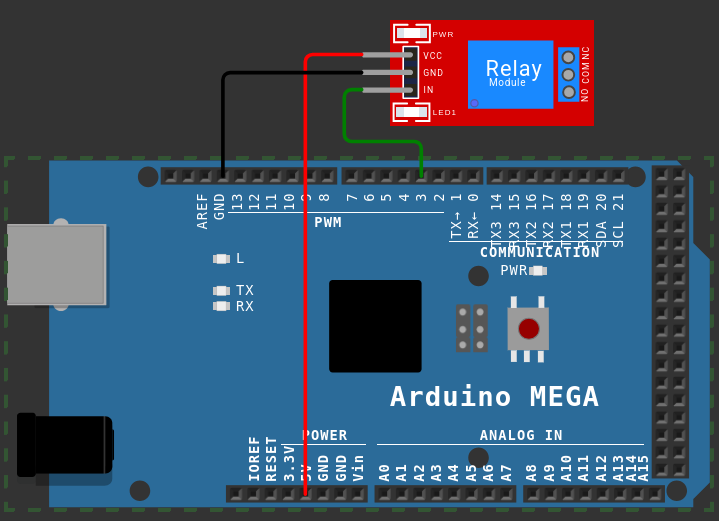
\includegraphics[width=0.45\textwidth]{images/relay_wokwi.png}
	\caption{Rangkaian simulasi modul relai daya satu saluran terisolasi optik pada platform Wokwi.}
	\label{fig:jqc3ff_module_image}
\end{figure}

Rincian pemetaan koneksi fisik antara pin modul relai JQC-3FF-S-Z dan periferal mikrokontroler ATmega2560 dirangkum pada Tabel~\ref{tab:jqc3ff_mcu_mapping}.

\begin{table}[H]
	\centering
	\caption{Pemetaan antarmuka modul relai JQC-3FF-S-Z ke Arduino Mega 2560}
	\label{tab:jqc3ff_mcu_mapping}
	\small
	\begin{tabularx}{\textwidth}{@{} p{3.5cm} p{3.8cm} X @{}}
		\toprule
		Kebutuhan Komponen         & Fitur MCU                         & Alasan Pemilihan \& Fungsi                                                                             \\
		\midrule
		Sinyal Pemicu Kontrol      & Pin GPIO Digital 3                & Mengirimkan sinyal tingkat logika biner untuk menyalakan atau mematikan relai                          \\
		Isolasi dan Penggerak Daya & Driver \textit{Optocoupler} PC817 & Mengisolasi pin GPIO MCU dari lonjakan tegangan serta arus induksi koil relai                          \\
		Catu Daya Koil Relai       & Rel Daya $5\,\text{V}$ \& GND MCU & Menyediakan pasokan tegangan ter-regulasi $5\,\text{V DC}$ dan arus $\approx 70\,\text{mA}$ untuk koil \\
		\bottomrule
	\end{tabularx}
\end{table}

\paragraph{Kode Demo Pengujian}
Berikut adalah implementasi kode program C++ untuk menguji fungsi sakelar relai daya secara periodik pada Arduino Mega 2560:

\begin{lstlisting}[language=C++, caption={Kode program pengujian sakelar relai JQC-3FF-S-Z pada Arduino Mega 2560}, label={lst:jqc3ff_code}]
#define RELAY_PIN 3

void setup() {
  Serial.begin(9600);
  Serial.println(F("Inisialisasi Pengujian Relai JQC-3FF..."));

  pinMode(RELAY_PIN, OUTPUT);
  digitalWrite(RELAY_PIN, HIGH);
}

void loop() {
  digitalWrite(RELAY_PIN, LOW);
  Serial.println(F("[AKTIF] Relai ON (Kontak COM-NO Terhubung)"));
  delay(3000);

  digitalWrite(RELAY_PIN, HIGH);
  Serial.println(F("[MATI] Relai OFF (Kontak COM-NO Terputus)"));
  delay(3000);
}
\end{lstlisting}

\paragraph{Gambaran Hasil Pembacaan}
Tampilan log keluaran pada \textit{Serial Monitor} saat simulasi eksekusi pengujian relai berjalan adalah sebagai berikut:

\begin{verbatim}
Inisialisasi Pengujian Relai JQC-3FF...
[AKTIF] Relai ON (Kontak COM-NO Terhubung)
[MATI] Relai OFF (Kontak COM-NO Terputus)
[AKTIF] Relai ON (Kontak COM-NO Terhubung)
\end{verbatim}
